\documentclass[UTF8]{ctexart}
\usepackage{mathtools,wallpaper}
\usepackage{listings}
\usepackage{t1enc}
\usepackage{pagecolor}
\usepackage{geometry}
\usepackage{diagbox}
\usepackage{CJK}
\usepackage{graphicx}
\usepackage{wrapfig}
\usepackage{amssymb}
\newcommand{\song}{\CJKfamily{song}}
\newcommand{\xiaoer}{\fontsize{18pt}{18pt}\selectfont}
\newcommand{\sanhao}{\fontsize{16pt}{16pt}\selectfont}
\newcommand{\sihao}{\fontsize{14pt}{24pt}\selectfont}
\geometry{left=2cm,right=2cm}

\linespread{1.7}
\geometry{left=3.18cm,right=3.18cm,top=2.54cm,bottom=2.54cm}
\setlength{\parindent}{0pt}
\begin{document}
\CTEXsetup[format={\Large\bfseries}]{section}
\begin{center}
    \song\xiaoer\textbf{中国科学技术大学计算机学院} \\
    \song\xiaoer\textbf{《数字电路实验》报告} \\
    \ \\
    \ \\
    \ \\
    
\includegraphics{school.jpg} \\
    \ \\
    \ \\
    \song\sanhao 实验题目:Logisim 入门 \\
    \song\sanhao 学生姓名:徐亦昶 \\
    \song\sanhao 学生学号: PB20000156\\
    \song\sanhao 完成日期: 2021.10.21\\
    \ \\
    \ \\
    \song\sihao 计算机实验教学中心制 \\
    \song\sihao 2020年09月
\end{center}
\newpage
\song\sihao
【实验题目】
\newline
Logisim 入门
\newline
【实验目的】
\newline
\begin{enumerate}
    \item 能够自行搭建 Logisim 实验环境
    \item 熟悉 Logisim 的各种基础器件和基本操作
    \item 能够使用 Logisim 搭建组合逻辑电路并进行仿真
    \item 能够使用封装子电路并进行电路设计
\end{enumerate}
【实验环境】
\newline
Linux 2.6.32、Logism 2.7.1
\newline
【实验过程】
\newline
由于配置环境和熟悉界面是进行实验的前提条件,这里直接从Step3开始写起。
\newline
Step 3:
\newline
1、常见器件及使用方式
\newline
\begin{enumerate}
    \item wire: 按钮,使用时将其在画布上连接即可,一根导线最多可以手动控制拐一个弯,使用时软件会自动控制其走向。
    \item pin: 分为输入和输出接口,对应属性选项卡中的output。可以设置Data Bits来改变端口的位宽,同时应改变facing使其朝向自然。
    \item probe: 探针,可以自动检测线上的数据,并以设置好的方法表示出来。
    \item splitter: 分线器,Fan Out表示分成几部分,Bit Width表示输入位宽,后面的每个Bit可取0到Fan Out-1个值,表示相应的位被分到那一部分。
    \item Gates: 常见逻辑门。
    \item Button: 按钮。
    \item LED/LED Matrix: LED灯或点阵。
    \item Constant: 用于给输入端口赋常量值,程序重新打开时不会变。
    \item Power/Ground: 高电平或接地。
    \item Poke Tool: 给端口赋值。
\end{enumerate}
2、实验结果
\begin{figure}[h!]
    \centering
    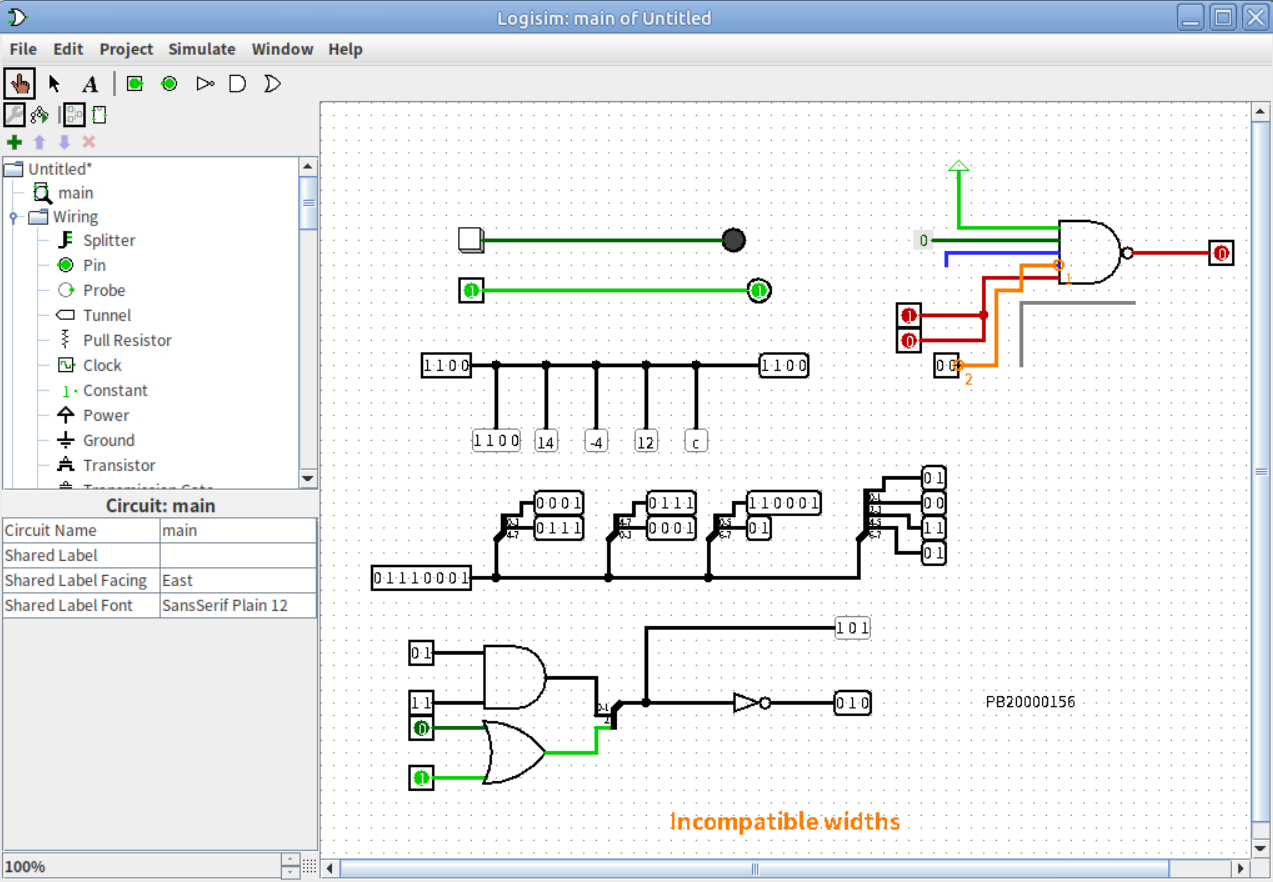
\includegraphics[scale=0.6]{step3.PNG}
    \caption{界面截图}
\end{figure}
\begin{figure}[h!]
    \centering
    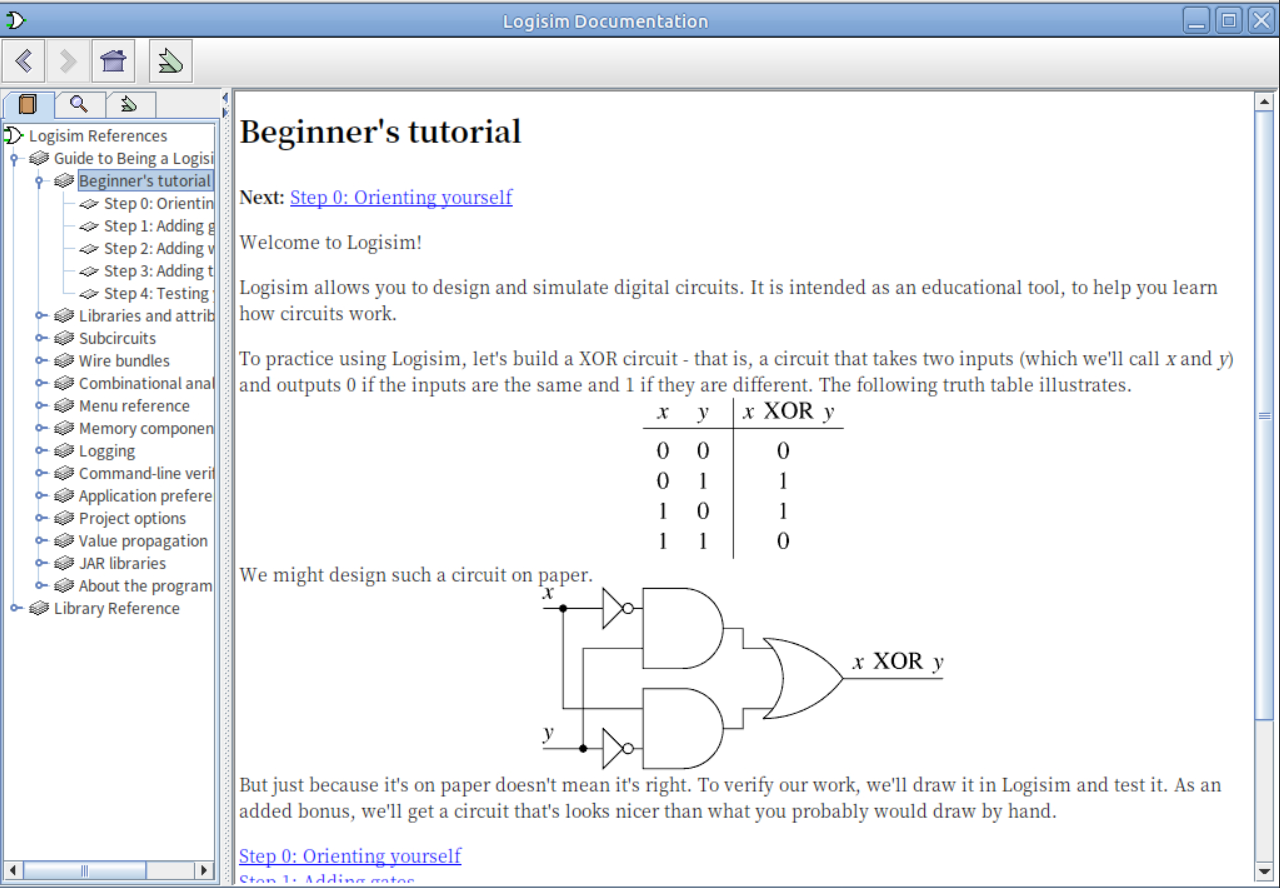
\includegraphics[scale=0.6]{tutor.PNG}
    \caption{使用文档}
\end{figure}
\newline
Step 4:
\newline
按照实验文档逐步搭建电路,每步截图如下:
\begin{figure}[h!]
    \centering
    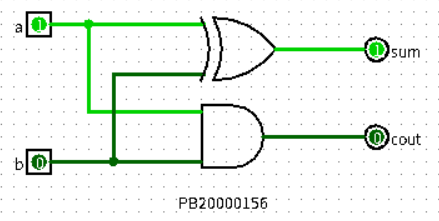
\includegraphics[scale=0.6]{S4_1.PNG}
    \caption{Step4 设计半加器}
\end{figure}
\begin{figure}[h!]
    \centering
    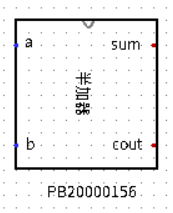
\includegraphics[scale=0.6]{S4_2.PNG}
    \caption{Step4 电路封装}
\end{figure}
\begin{figure}[h!]
    \centering
    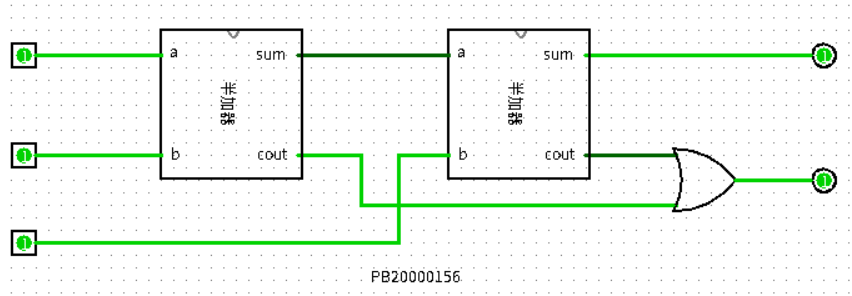
\includegraphics[scale=0.6]{S4_3.PNG}
    \caption{Step4 全加器}
\end{figure}
\newline
【实验练习】
\newline
\textbf{第一题\ LED点阵}
\newline
1、在左侧的组件中找到LED Matrix,调整行数和列数分别为16,使用16个Constant给每个引脚赋值,将Constant组件的Data Bits设为16,并
拖放到合适的位置排成一列。
\begin{figure}[h!]
    \centering
    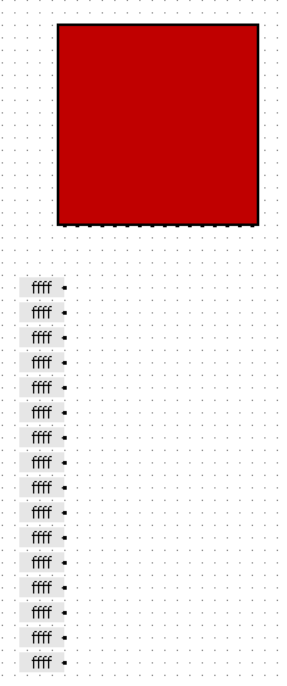
\includegraphics[scale=0.6]{p1_s1.PNG}
    \caption{第一题第一步}
\end{figure}
\newline
2、连线
\begin{figure}[h!]
    \centering
    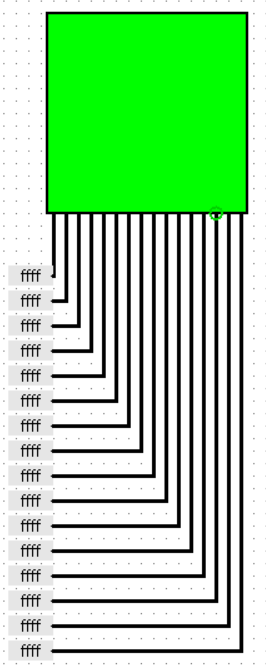
\includegraphics[scale=0.6]{p1_s2.PNG}
    \caption{第一题第二步}
\end{figure}
\newline
3、将该电路复制成三份,并从左到右依次摆放。
\begin{figure}[h!]
    \centering
    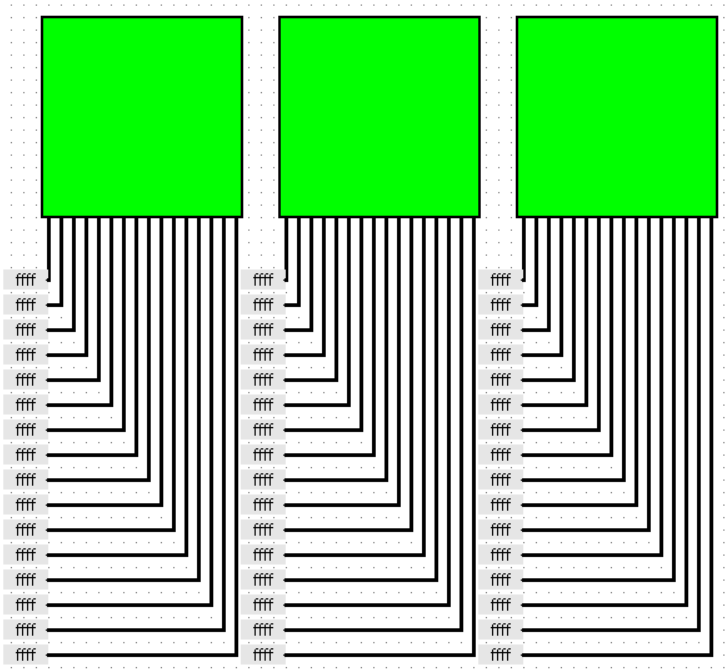
\includegraphics[scale=0.6]{p1_s3.PNG}
    \caption{第一题第二步}
\end{figure}
\newline
4、使用js脚本将汉字分解为点阵
\begin{figure}[h!]
    \centering
    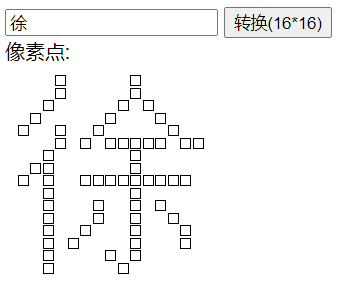
\includegraphics[scale=0.6]{name_mat.PNG}
    \caption{汉字点阵}
\end{figure}
\newline
注意后面的二进制矩阵应该按列转换成16进制,因此需要写一个程序,将矩阵转置后输出。
\begin{figure}[h!]
    \centering
    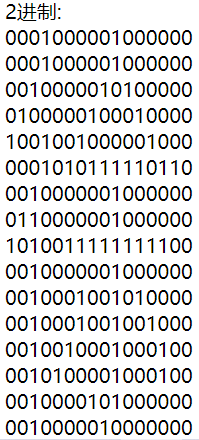
\includegraphics[scale=0.6]{name_mat_bin.PNG}
    \caption{二进制矩阵}
\end{figure}
\newline
\begin{lstlisting}[language={c++},numbers=left,numberstyle=\tiny,%frame=shadowbox,  
       rulesepcolor=\color{red!20!green!20!blue!20},  
       keywordstyle=\color{blue!70!black},  
       commentstyle=\color{blue!90!},  
       basicstyle=\ttfamily] 
#include<iostream>
using namespace std;
int main()
{
	char mat[16][16];
	for(int i=0;i<16;i++) cin>>mat[i];
	system("cls");
	for(int i=0;i<16;i++)
	{
		for(int j=0;j<16;j++)
			cout<<mat[j][i];
		cout<<endl;
	}
	return 0;
 } 
\end{lstlisting}
再使用Python脚本将每一行的二进制转换成16进制:
\begin{lstlisting}[language={python},numbers=left,numberstyle=\tiny,%frame=shadowbox,  
    rulesepcolor=\color{red!20!green!20!blue!20},  
    keywordstyle=\color{blue!70!black},  
    commentstyle=\color{blue!90!},  
    basicstyle=\ttfamily]
a=[]
for i in range(0,16):
    a.append(input())
for i in range(0,16):
    print(hex(int(a[i],2)))
\end{lstlisting}
最后,给LED点阵赋值:
\begin{figure}[h!]
    \centering
    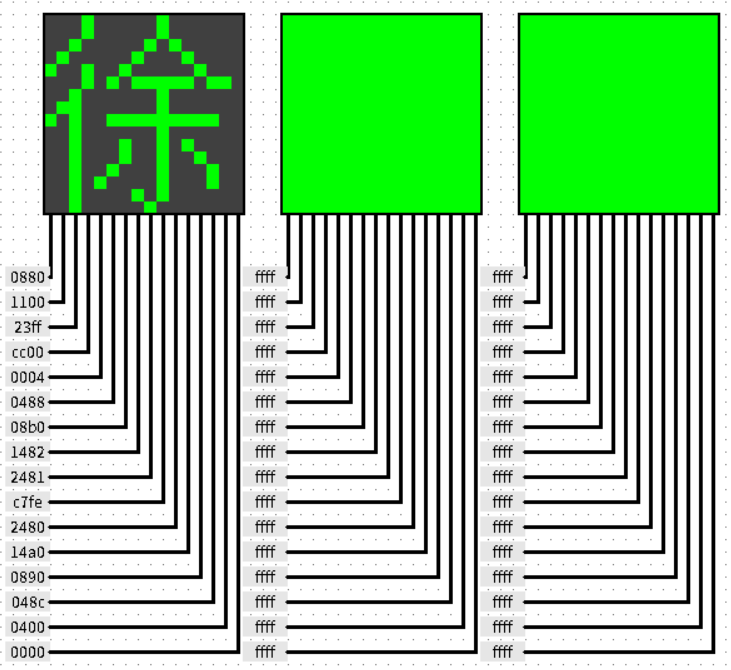
\includegraphics[scale=0.6]{p1_s4.PNG}
    \caption{第一题 LED点阵赋值}
\end{figure}
\newline
最终结果:
\begin{figure}[h!]
    \centering
    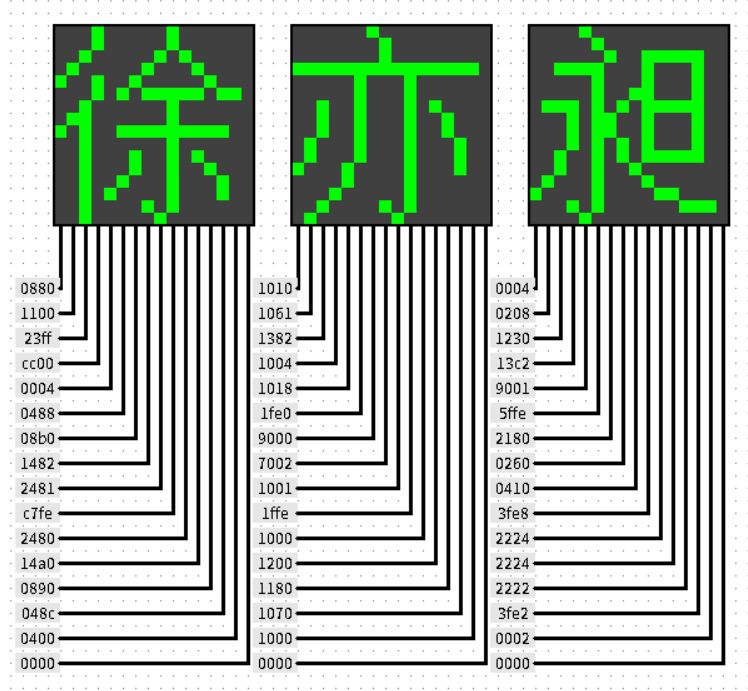
\includegraphics[scale=0.6]{p1.PNG}
    \caption{第一题 最终结果}
\end{figure}
\newline
\textbf{第二题\ 七段数码管}
\newline
1、在左侧的组件中找到7-Segment Display,布置相应的Pin为输入端口并进行布线。
\begin{figure}[h!]
    \centering
    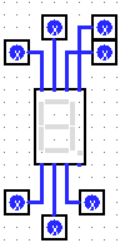
\includegraphics[scale=0.6]{p2_s1.PNG}
    \caption{第二题 设置单个数码管}
\end{figure}
\newline
2、将数码管复制,排成一排。
\begin{figure}[h!]
    \centering
    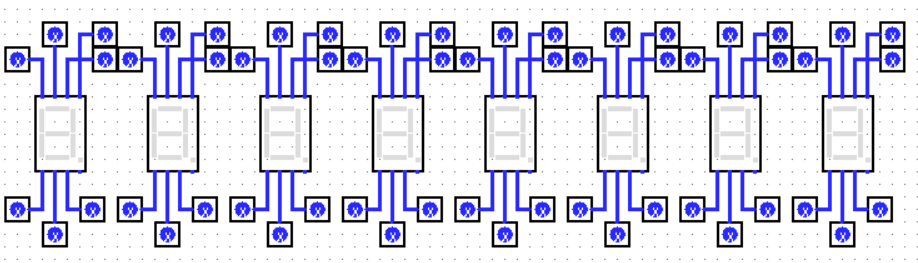
\includegraphics[scale=0.6]{p2_s2.PNG}
    \caption{第二题 复制数码管}
\end{figure}
\newline
3、将阴极接地,形成共阴数码管。
\begin{figure}[h!]
    \centering
    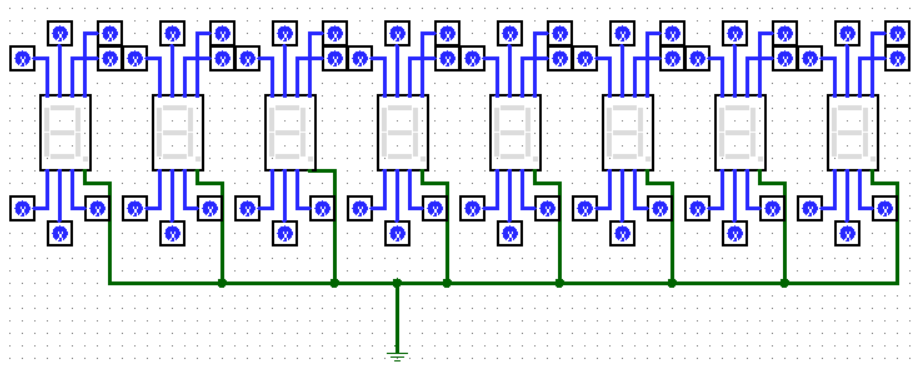
\includegraphics[scale=0.6]{p2_s3.PNG}
    \caption{第二题 阴极接地}
\end{figure}
\newline
4、开启poke模式,依次点亮每一段。
\begin{figure}[h!]
    \centering
    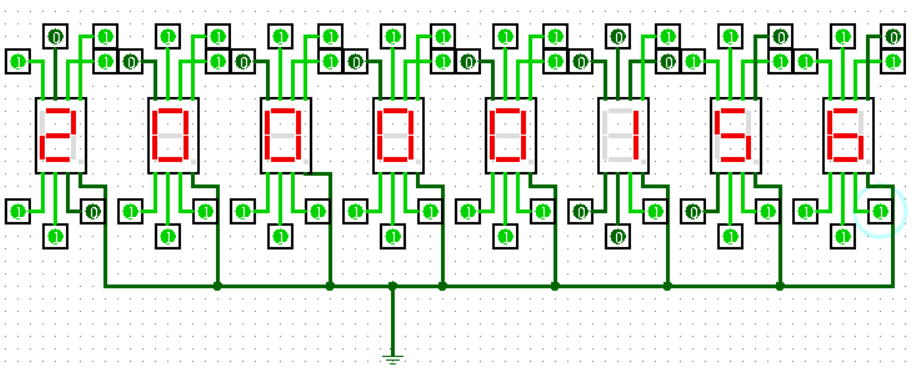
\includegraphics[scale=0.6]{p2.PNG}
    \caption{第二题 最终结果}
\end{figure}
\newline
\textbf{第三题\ MOS}
\newline
1、以与门为例,第一步先将晶体管和端口排列好,可通过Type调整晶体管的类型(P型或N型),
以及Facing调节晶体管朝向。
\begin{figure}[h!]
    \centering
    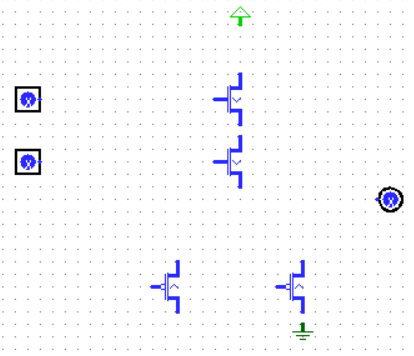
\includegraphics[scale=0.6]{p3_s1.PNG}
    \caption{第三题 摆放组件}
\end{figure}
\newline
2、连线。
\begin{figure}[h!]
    \centering
    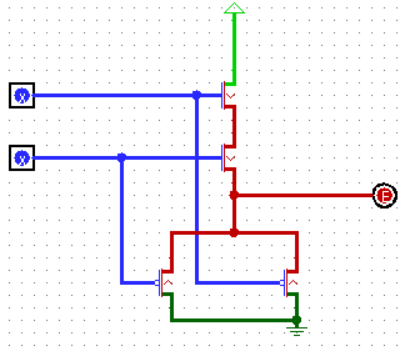
\includegraphics[scale=0.6]{p3_s2.PNG}
    \caption{第三题 连线}
\end{figure}
\newline
类似搭建其余两种门,最终结果如下:
\begin{figure}[h!]
    \centering
    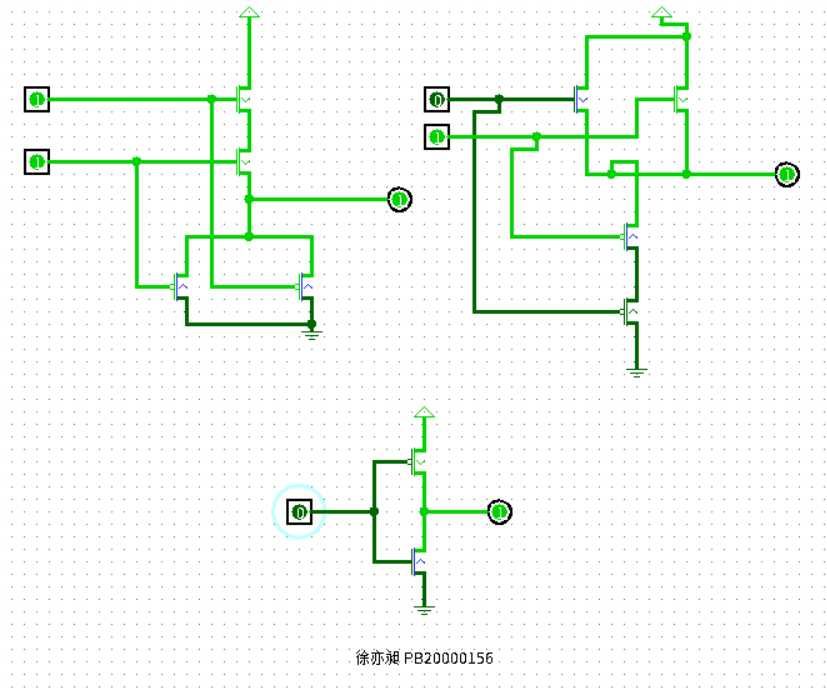
\includegraphics[scale=0.6]{p3.PNG}
    \caption{第三题 最终结果}
\end{figure}
\newline
\textbf{第四题\ 数据选择器}
\newline
1、添加电路,分别将上题中的三种门封装。
\begin{figure}[h!]
    \centering
    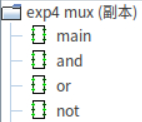
\includegraphics[scale=0.6]{p4_s1.PNG}
    \caption{第四题 封装}
\end{figure}
\newline
2、设计二选一数据选择器,用到两个与门、一个非门、一个或门。
\begin{figure}[h!]
    \centering
    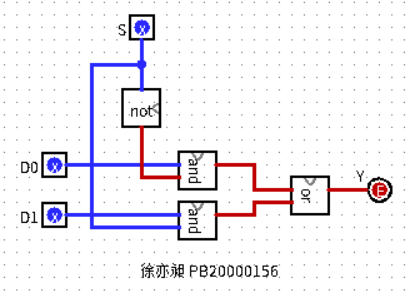
\includegraphics[scale=0.6]{p4_s2.PNG}
    \caption{第四题 二选一数字选择器}
\end{figure}
\newline
3、将位宽改为2。
\begin{figure}[h!]
    \centering
    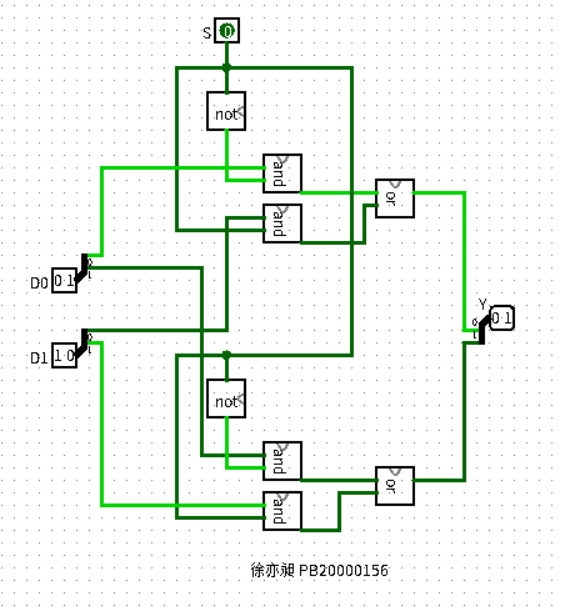
\includegraphics[scale=0.6]{p4_s3.PNG}
    \caption{第四题 位宽改为2}
\end{figure}
\newline
4、新建电路,取名为mux,将上述二选一选择器放入并封装。最后的文件系统如图所示:
\begin{figure}[h!]
    \centering
    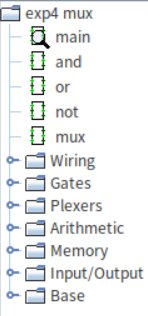
\includegraphics[scale=0.6]{p4_files.PNG}
    \caption{第四题 文件系统}
\end{figure}
\newline
5、设计四选一选择器,用到六个与门、三个非门、三个或门。
\begin{figure}[h!]
    \centering
    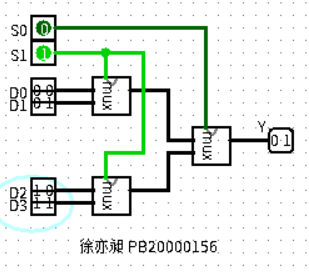
\includegraphics[scale=0.6]{p4.PNG}
    \caption{第四题 四选一选择器}
\end{figure}
\newline
【总结与思考】
\newline
1、通过本次实验,掌握了Logisim的基本用法,如电路的创建、模拟、封装等;
通过具体的实践,对电路的设计有了更深的认识。
\newline
2、难度适中,可能不容易上手,但一旦上手可以很快完成。
\newline
3、任务量较大,比如前面的步骤4完全不必设计这么多电路,很多可以在后面的实验中学到。
\newline
4、建议以“学会为止”设计实验,比如练习题第一题让LED点阵显示自己的姓即可。
\end{document}